\documentclass[11pt]{article}
\usepackage{graphicx}
\usepackage{hyperref}
\begin{document}
\title{Final Report}
\author{Yafie Qu\hspace{10 mm}TCD\\Hao Guan\hspace{10 mm}TCD\\Jeremiah Dunn\hspace{10 mm}TCD\\Saloni Sharma\hspace{10 mm}14327635\\CS7038: Group Project\\School of Computer Science and Statistics\\Trinity College Dublin\\
\includegraphics[scale=1.5]{TCD.jpg}}
\maketitle
\section{Overview of the Project}
\subsection{Background Story}
The story of the game is about a space expedition. Our player is on a long journey and space ship begins malfunctioning. Different subsystems start failing and security system begins to malfunction. The whole crew of the ship is in stasis and unaware of the situation. The player controls the maintenance droid.  This maintenance droid is the only unaffected robot or computer on the ship. His task is to restore power to ship's subsystem and fixing the security system. Now the ship's fate is in the hands of this humble maintenance droid.
\subsection{Theme}
This is the International Year of Light and Light-based Technologies, 2015. This is a United Nations observance that aims to raise awareness of the achievements of light science and its applications and importance.\\

This game accounts this year's theme of light. When the space ship is wrecked and malfunctions, it looses all its power sources and light. Our maintenance robot switches on the power and brings back light to each room of each part of the space ship during the game-play.\\

Different part(level) of the ship begin dark. As our droid explores the level, he returns power to different components. As the components turned on, the ship begins to lit back up. 
\subsection{Initial Design}
This is an exploration based platformer 2D game. The initial design focused on the randomised level generation. This aspect of the game-play is inspired from an exploration based platformer games such as \textit{Spelunky}.\\

The game-play also aimed at the dynamic lighting system which changes the appearance of the ship. These dynamic lighting effects are generated  using placement of point, spot lights and normal maps for different game objects.
\section{Technical Overview}
The game is made using \textit{Unity}. Game physics are implemented using Unity 2D physics engine. Normal maps and height maps are generated using \textit{SpriteLamp} and \textit{Crazy Bump}.
\subsection{Level Generation}
Each level begins with a 2D grid of an arbitrary size. \textit{Solution Path} is then generated through the level. In figure 1, First a point on the top of the grid is chosen to the start of the level. We then can step through the grid towards the bottom. Now a left/right is chosen randomly. There is then a random chance of stepping in this direction or stepping down. After stepping down, we chose our random direction again and repeat the process. When we reach the bottom floor the down probability is replaced by a probability of choosing the exit.\\

We then assign one of the different room types to each point on the \textit{Solution Path}. These room types correspond to the exits/entrances that each room needs. After this, we draw a boundary around the level. This way we can create a level using four different categories of exit types.

\begin{figure}[!htb]\centering
   \begin{minipage}{0.49\textwidth}
     \frame{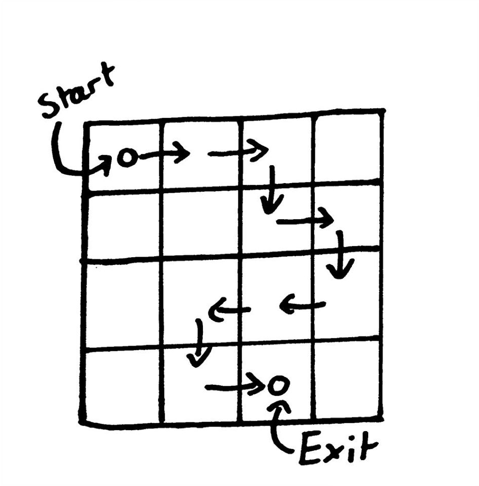
\includegraphics[width=\linewidth]{levelgen1.png}}
     \caption{Solution Path Generation}\label{Fig:Data1}
   \end{minipage}
   \begin {minipage}{0.49\textwidth}
     \frame{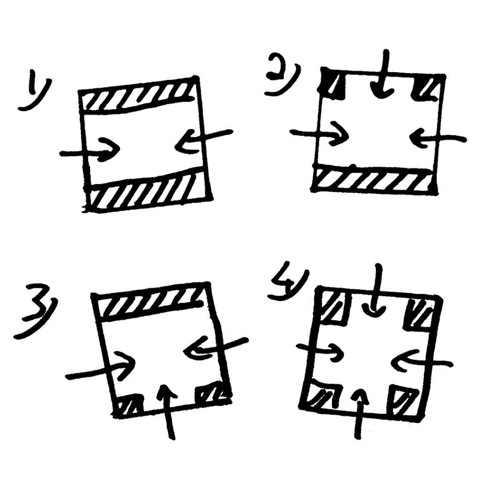
\includegraphics[width=\linewidth]{levelgen2.png}}
     \caption{Room Types}\label{Fig:Data2}
   \end{minipage}
\end{figure}

\subsection{Rooms}
Rooms are 16x16 grids of tiles, there are different rooms for different exit types. Room is initially created as a comma separated text file. The game reads in the text files. During level generation, these text files with appropriate exit types are randomly chosen to fill in the level.\\

In the text files, the different letters represent different tile types such as solid, lights with radii, traps, etc. These can be easily swapped out of the game to create and text new levels.

\begin{figure}[!htb]\centering
   \begin{minipage}{0.49\textwidth}
     \frame{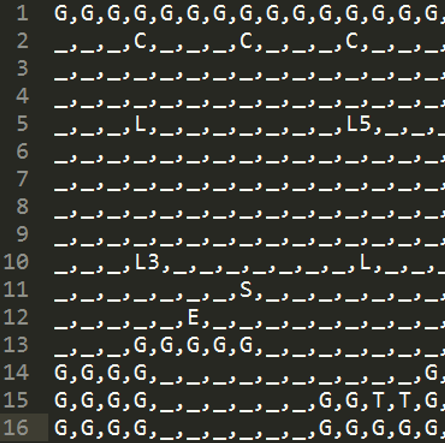
\includegraphics[width=\linewidth]{room.png}}
     \caption{Input text file}\label{Fig:Data1}
   \end{minipage}
   \begin {minipage}{0.49\textwidth}
     \frame{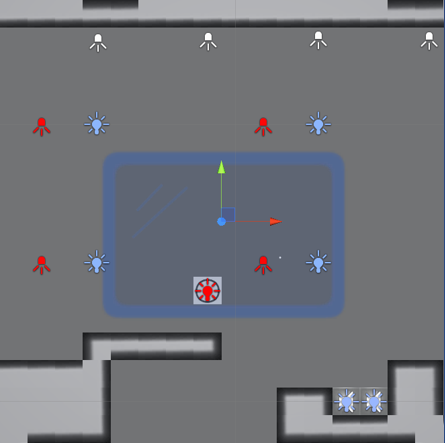
\includegraphics[width=\linewidth]{room1.png}}
     \caption{Unity Editor Output}\label{Fig:Data2}
   \end{minipage}
\end{figure}

\subsection{Lighting System}
\subsection{Security System}
\subsection{Player Character}
\section{Team Organisation}
Scrum has been used for the product development which is an iterative and incremental agile software development methodology for managing product development.\\

The team has used Jira for project management and Git as a repository for synchronised progress across team and for  maintaining development using stable branches.\\

The team created high level overview of tasks called as Epics. The game project idea is divided into these Epics: \textit{Level Generation}, \textit{GUI}, \textit{Core Game} and \textit{Character Controller}.\\

These Epics were further broke down into smaller and manageable tasks called as Stories. The project was divided into 4 sprints. Each sprint lasted for 2 weeks. At start of each sprint, team had regular grooming sessions to estimate and re-estimate the stories and their implementation time. Task for each sprint will be chosen from the backlog based on their priority and requirements. In the grooming sessions, team looked through the backlog and see what stories they want to work on, assign story points, give them time estimates and flesh-out the descriptions or sub-task them as required. Time estimation for different tasks has been carried off by using voting system and then taking average of individual estimated time.\\

Team had regular stand-ups, an average of thrice a week. Stand-ups were aimed to last for 10 minutes with any additional discussions happened in separate meeting outside this time.\\

Team prioritized the project stories by keeping Level generation and core game on high priority and GUI on the least priority. This was implemented for an organized way of development so that major game-play could be implemented on time keeping an account of time spent on other assignments of coursework. During the course of project, team learned more about Unity and skills/efficiency of different team members.

\section{Conclusion}

\section{You Tube Link}

\section{Acknowledgements}

\end{document}